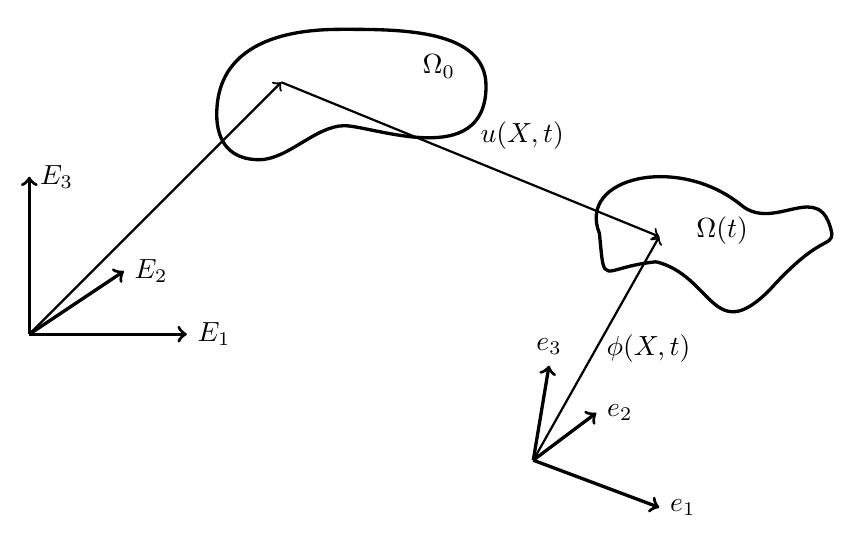
\begin{tikzpicture}[scale=0.8]
  %\draw[step=1.0,black,thin] (-3.,-1.) grid (3,4.);
  %\draw (-3,-1) -- (3,-1) -- (3,4) -- (-3,4) -- (-3,-1);
  \draw[very thick,->] (-5,-2.5) -- (-2.5,-2.5) node [right] {$\vect{E}_1$};
  \draw[very thick,->] (-5,-2.5) -- (-5,0.) node [right] {$\vect{E}_3$};
  \draw[very thick,->] (-5,-2.5) -- (-3.5,-1.5) node [right] {$\vect{E}_2$};
  \draw[very thick,->] (3,-3.5-1.) -- (5.,-4.25-1.) node [right] {$\vect{e}_1$};
  \draw[very thick,->] (3,-3.5-1.) -- (3.25,-2.-1.) node [above] {$\vect{e}_3$};
  \draw[very thick,->] (3,-3.5-1.) -- (4.,-2.75-1.) node [right] {$\vect{e}_2$};
  \begin{scope}[scale=0.45]
    \draw[very thick] (-3,0.6) .. controls +(1,0) and +(-1,0) .. (0,1.8)  
    .. controls +(1,0) and +(0,-3) .. (5,3.2) 
    .. controls +(0,2) and +(2,0)  .. (0,5.2) 
    .. controls +(-1,0) and +(0,3) .. (-4.5,2.2) 
    .. controls +(0,-1) and +(-1,0).. (-3,0.6) ;
  \end{scope}
  \node at (1.5,1.75) {$\Omega_0$};
  %% Deformed body +2.
  \begin{scope}[scale=0.9]
    \draw[very thick] (0.+0.5+5.,0-1.5) ..controls (1.+0.5+5.,-0.25-1.5) and (1.+0.5+5.,-1.5-1.5) .. (2.+0.5+5.,-0.5-1.5) ..controls (2.9+0.5+5.,0.5-1.5) and (3.1+0.5+5.,0.25-1.5) .. (3.1+0.5+5.,0.5-1.5) ..controls (2.9+0.5+5.,1.5-1.5) and (2.1+0.5+5.,.5-1.5) .. (1.5+0.5+5.,1.-1.5) ..controls (0.4+0.5+5.,1.9-1.5) and (-1.4+0.5+5.,1.5-1.5) .. (-1.+0.5+5.,0.5-1.5)..controls (-0.4+0.+5.,-0.-2.) and (-1+0.5+5.,0.4-2.) .. (0+0.5+5.,0-1.5);
  \end{scope}
  \node at (6.,-0.85) {$\Omega(t)$};
  \draw[->,thick] (-5,-2.5) -- (-1.,1.5) node [midway,left] {$\X$};
  \draw[->,thick] (3,-3.5-1.) -- (5.,-0.95) node [midway,right] {$\vect{\phi}(\vect{X},t)$};
  \draw[->,thick] (-1.,1.5) -- (5.,-0.95) node [midway,above right] {$\vect{u}(\vect{X},t)$};
\end{tikzpicture}

%%% Local Variables:
%%% mode: latex
%%% TeX-master: "../../mainManuscript"
%%% End: